% Options for packages loaded elsewhere
\PassOptionsToPackage{unicode}{hyperref}
\PassOptionsToPackage{hyphens}{url}
\PassOptionsToPackage{dvipsnames,svgnames,x11names}{xcolor}
%
\documentclass[
]{article}

\usepackage{amsmath,amssymb}
\usepackage{iftex}
\ifPDFTeX
  \usepackage[T1]{fontenc}
  \usepackage[utf8]{inputenc}
  \usepackage{textcomp} % provide euro and other symbols
\else % if luatex or xetex
  \usepackage{unicode-math}
  \defaultfontfeatures{Scale=MatchLowercase}
  \defaultfontfeatures[\rmfamily]{Ligatures=TeX,Scale=1}
\fi
\usepackage{lmodern}
\ifPDFTeX\else  
    % xetex/luatex font selection
\fi
% Use upquote if available, for straight quotes in verbatim environments
\IfFileExists{upquote.sty}{\usepackage{upquote}}{}
\IfFileExists{microtype.sty}{% use microtype if available
  \usepackage[]{microtype}
  \UseMicrotypeSet[protrusion]{basicmath} % disable protrusion for tt fonts
}{}
\makeatletter
\@ifundefined{KOMAClassName}{% if non-KOMA class
  \IfFileExists{parskip.sty}{%
    \usepackage{parskip}
  }{% else
    \setlength{\parindent}{0pt}
    \setlength{\parskip}{6pt plus 2pt minus 1pt}}
}{% if KOMA class
  \KOMAoptions{parskip=half}}
\makeatother
\usepackage{xcolor}
\usepackage[top=30mm,left=20mm,right=20mm,bottom=30mm]{geometry}
\setlength{\emergencystretch}{3em} % prevent overfull lines
\setcounter{secnumdepth}{5}
% Make \paragraph and \subparagraph free-standing
\ifx\paragraph\undefined\else
  \let\oldparagraph\paragraph
  \renewcommand{\paragraph}[1]{\oldparagraph{#1}\mbox{}}
\fi
\ifx\subparagraph\undefined\else
  \let\oldsubparagraph\subparagraph
  \renewcommand{\subparagraph}[1]{\oldsubparagraph{#1}\mbox{}}
\fi


\providecommand{\tightlist}{%
  \setlength{\itemsep}{0pt}\setlength{\parskip}{0pt}}\usepackage{longtable,booktabs,array}
\usepackage{calc} % for calculating minipage widths
% Correct order of tables after \paragraph or \subparagraph
\usepackage{etoolbox}
\makeatletter
\patchcmd\longtable{\par}{\if@noskipsec\mbox{}\fi\par}{}{}
\makeatother
% Allow footnotes in longtable head/foot
\IfFileExists{footnotehyper.sty}{\usepackage{footnotehyper}}{\usepackage{footnote}}
\makesavenoteenv{longtable}
\usepackage{graphicx}
\makeatletter
\def\maxwidth{\ifdim\Gin@nat@width>\linewidth\linewidth\else\Gin@nat@width\fi}
\def\maxheight{\ifdim\Gin@nat@height>\textheight\textheight\else\Gin@nat@height\fi}
\makeatother
% Scale images if necessary, so that they will not overflow the page
% margins by default, and it is still possible to overwrite the defaults
% using explicit options in \includegraphics[width, height, ...]{}
\setkeys{Gin}{width=\maxwidth,height=\maxheight,keepaspectratio}
% Set default figure placement to htbp
\makeatletter
\def\fps@figure{htbp}
\makeatother

\usepackage{fancyhdr}
\pagestyle{fancy}
\fancyhead[R]{ENSGSI 2AP - Mécanique des Solidés Déformables}

\fancyfoot[L]{Guillaume PRONOST | Fabio CRUZ}
\fancyfoot[C]{\thepage}
\fancyfoot[R]{ENSGSI - 2023/2024}
\renewcommand{\footrulewidth}{0.3pt}% default is 0pt
\makeatletter
\makeatother
\makeatletter
\makeatother
\makeatletter
\@ifpackageloaded{caption}{}{\usepackage{caption}}
\AtBeginDocument{%
\ifdefined\contentsname
  \renewcommand*\contentsname{Table of contents}
\else
  \newcommand\contentsname{Table of contents}
\fi
\ifdefined\listfigurename
  \renewcommand*\listfigurename{List of Figures}
\else
  \newcommand\listfigurename{List of Figures}
\fi
\ifdefined\listtablename
  \renewcommand*\listtablename{List of Tables}
\else
  \newcommand\listtablename{List of Tables}
\fi
\ifdefined\figurename
  \renewcommand*\figurename{Figure}
\else
  \newcommand\figurename{Figure}
\fi
\ifdefined\tablename
  \renewcommand*\tablename{Table}
\else
  \newcommand\tablename{Table}
\fi
}
\@ifpackageloaded{float}{}{\usepackage{float}}
\floatstyle{ruled}
\@ifundefined{c@chapter}{\newfloat{codelisting}{h}{lop}}{\newfloat{codelisting}{h}{lop}[chapter]}
\floatname{codelisting}{Listing}
\newcommand*\listoflistings{\listof{codelisting}{List of Listings}}
\makeatother
\makeatletter
\@ifpackageloaded{caption}{}{\usepackage{caption}}
\@ifpackageloaded{subcaption}{}{\usepackage{subcaption}}
\makeatother
\makeatletter
\@ifpackageloaded{tcolorbox}{}{\usepackage[skins,breakable]{tcolorbox}}
\makeatother
\makeatletter
\@ifundefined{shadecolor}{\definecolor{shadecolor}{rgb}{.97, .97, .97}}
\makeatother
\makeatletter
\makeatother
\makeatletter
\makeatother
\ifLuaTeX
  \usepackage{selnolig}  % disable illegal ligatures
\fi
\IfFileExists{bookmark.sty}{\usepackage{bookmark}}{\usepackage{hyperref}}
\IfFileExists{xurl.sty}{\usepackage{xurl}}{} % add URL line breaks if available
\urlstyle{same} % disable monospaced font for URLs
\hypersetup{
  pdftitle={TD 1: Introduction},
  colorlinks=true,
  linkcolor={blue},
  filecolor={Maroon},
  citecolor={Blue},
  urlcolor={Blue},
  pdfcreator={LaTeX via pandoc}}

\title{TD 1: Introduction}
\usepackage{etoolbox}
\makeatletter
\providecommand{\subtitle}[1]{% add subtitle to \maketitle
  \apptocmd{\@title}{\par {\large #1 \par}}{}{}
}
\makeatother
\subtitle{Objectif: Application de la Loi de Hooke}
\author{}
\date{}

\begin{document}
\maketitle
\ifdefined\Shaded\renewenvironment{Shaded}{\begin{tcolorbox}[sharp corners, frame hidden, boxrule=0pt, enhanced, borderline west={3pt}{0pt}{shadecolor}, breakable, interior hidden]}{\end{tcolorbox}}\fi

\thispagestyle{fancy}

\hypertarget{exercise-1-contrainte-en-traction}{%
\section{Exercise 1: Contrainte en
traction}\label{exercise-1-contrainte-en-traction}}

Soit une force \(F\) de 1440 \(kN\) à une tige de longeur initiale de
4\(m\). Cette tige a une section carré de \(20cm \times 20cm\) et
s'allonge de \(2mm\). Le matériaux est à determiner.

\begin{figure}

\begin{minipage}[c]{0.35\linewidth}

{\centering 

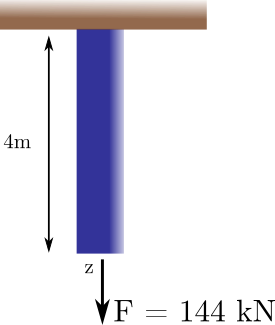
\includegraphics[width=4.2cm,height=\textheight]{../assets/img/TD1/Ex1.png}

}

\end{minipage}%
%
\begin{minipage}[c]{0.65\linewidth}

{\centering 

\begin{enumerate}
\def\labelenumi{\arabic{enumi}.}
\item
  Calculez la déformation normale \(\epsilon\), la contrainte en
  traction \(\sigma\) et son module de Young d'elasticité \(E\).
\item
  A quel matériau pur ce module de Young peut-il correspondre ?
\end{enumerate}

}

\end{minipage}%

\end{figure}

\hypertarget{exercise-2-contrainte-de-cisallement}{%
\section{Exercise 2: Contrainte de
Cisallement}\label{exercise-2-contrainte-de-cisallement}}

\begin{figure}

\begin{minipage}[c]{0.40\linewidth}

{\centering 

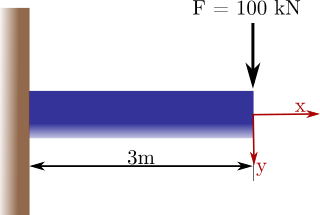
\includegraphics[width=5cm,height=\textheight]{../assets/img/TD1/Ex2.png}

}

\end{minipage}%
%
\begin{minipage}[c]{0.60\linewidth}

{\centering 

Calculez la déformation tangentielle (demi distorsion angulaire) d'une
tige d'alluminium de \(3~m\) de long et de \(1~cm^{2}\) de section qui
est soumise à un effort transversal de \(100~kN\)

}

\end{minipage}%

\end{figure}

\hypertarget{exercise-3-compression-poteau}{%
\section{Exercise 3: Compression
poteau}\label{exercise-3-compression-poteau}}

Un poteau de chêne (module de Young \(E= 12~GPa\)) de \(3~m\) est
utilisé pour supporter une charge compressive dans le sens des fibres.
La section du poteau est carrée et vaut \(235~mm \times 235~mm\). Une
masse de \(20~kg\) est appliquée sur la partie supérieure du poteau.

\begin{enumerate}
\def\labelenumi{\arabic{enumi}.}
\tightlist
\item
  Calculer la valeur de la \emph{contrainte normale} imposée par la
  masse ?
\item
  En déduire la valeur de la \emph{déformation normale} ?
\item
  Quelle est la valeur de la longueur lorsque le poteau est déformé ?
\end{enumerate}

\hypertarget{exercise-4-analysuxe9-de-lessaie-de-traction}{%
\section{Exercise 4: Analysé de l'essaie de
traction}\label{exercise-4-analysuxe9-de-lessaie-de-traction}}

Un test de traction est réalisé sur une éprouvette parallélépipède de
longueur \(L_{0}= 10~cm\) et de section \(4~cm^{2}\).

\begin{figure}

\begin{minipage}[c]{0.50\linewidth}

{\centering 

Le matériau considéré est \emph{fragile} et l'essai est effectué jusqu'à
la rupture sur une éprouvette parallélépipédique. La courbe de l'essai
de traction représenté par la force F en fonction de l'allongement
\(\Delta L\) est présentée ci-dessous :

}

\end{minipage}%
%
\begin{minipage}[c]{0.50\linewidth}

{\centering 

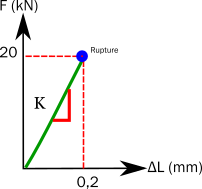
\includegraphics[width=5cm,height=\textheight]{../assets/img/TD1/Ex4.png}

}

\end{minipage}%

\end{figure}

\begin{enumerate}
\def\labelenumi{\arabic{enumi}.}
\tightlist
\item
  Déterminer la \emph{rigidité} de la structure de l'éprouvette.
\item
  D'après la courbe \(F=f(\Delta L)\), déterminer la courbe de
  contrainte \(\sigma\) en fonction de la déformation \(\epsilon\), puis
  déterminer la valeur du module de Young ainsi que le matériau associé
  ?
\item
  Soit une éprouvette composée du même matériau, de même longueur mais
  de section deux fois supérieure.
\end{enumerate}

\begin{itemize}
\tightlist
\item
  Tracer la contrainte en fonction de la déformation ainsi que la force
  en fonction de l'allongement.
\item
  Tracer sur les mêmes graphiques avec cette fois-ci une éprouvette de
  même section mais de longueur double \(L_{0}= 20~cm\).
\end{itemize}

\begin{enumerate}
\def\labelenumi{\arabic{enumi}.}
\setcounter{enumi}{3}
\tightlist
\item
  Exprimer la relation reliant rigidité de la structure avec la section,
  la longueur de l'éprouvette et le module de Young peut être déduite.
\end{enumerate}



\end{document}
